\section{Motivating Examples}

Analytical modeling is difficult for many code sequences; consider examples (a)-(c), their actual throughput\footnote{Note that -- following convention -- we define throughput to be the number of clock cycles taken to execute a basic block; this is actually the reciprocal of the standard definition of throughput. We also report throughput for 100 iterations of a given basic block.}, and their associated throughput predictions in Table~\ref{tbl:motivation}.
These flawed predictions occur in spite of many hours spent engineering detailed models of underlying microarchitectural details.
In contrast, \tool{}'s data driven approach intrinsically learns accurate predictions from the ground truth data.

\begin{table}[h!]
  \centering
  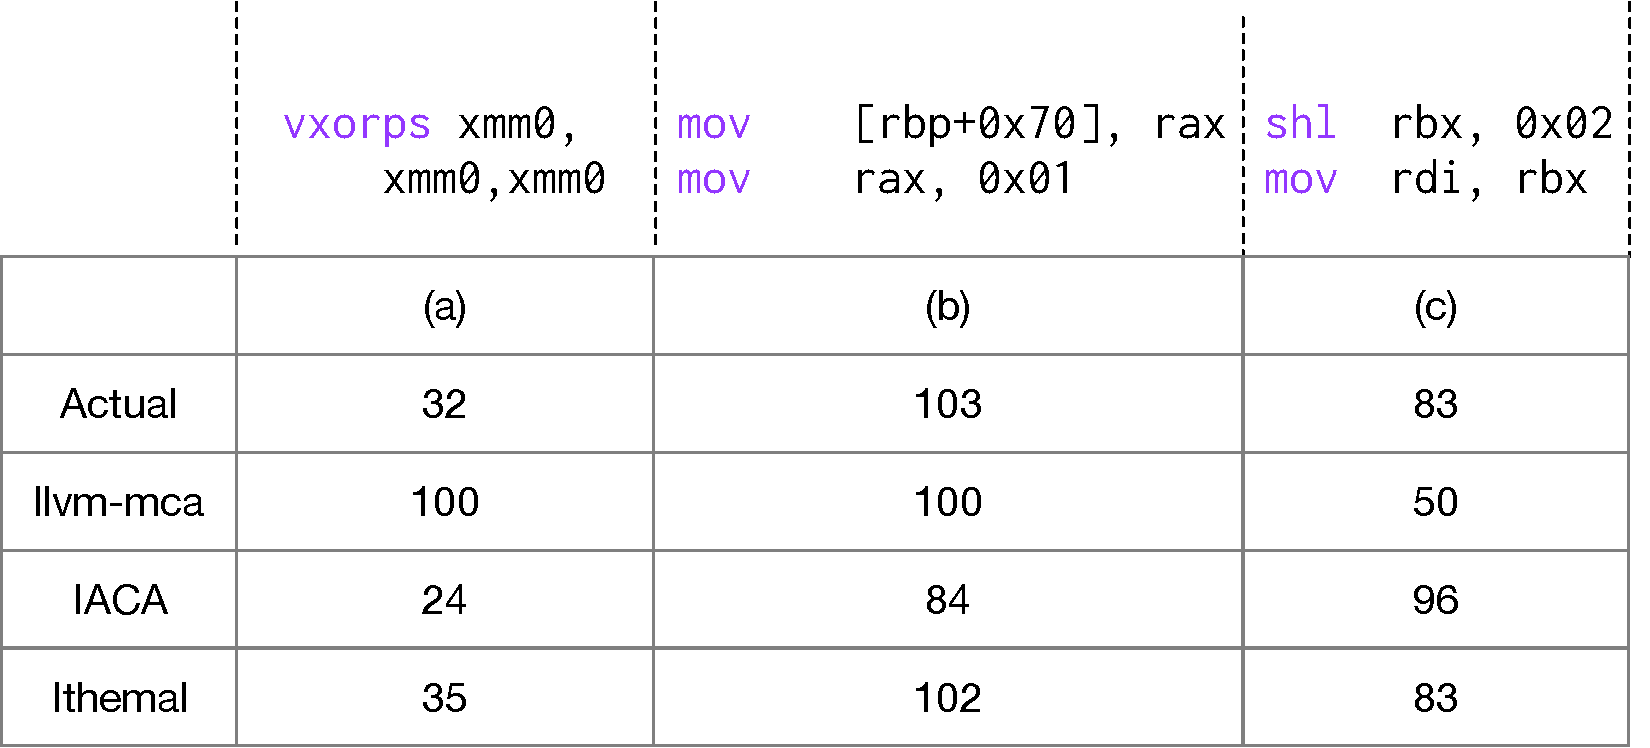
\includegraphics[width=\columnwidth]{figures/motivation-examples.pdf}
  \vspace{-20pt}
  \caption{Example x86-64 assembly code sequences (Intel syntax) and associated throughput predictions, in clock cycles}
  \label{tbl:motivation}
\end{table}

% This is the full system architecture diagram, which LaTeX won't place nicely unless it's all the way on the previous page
\begin{figure*}[ht!]
  \centering
  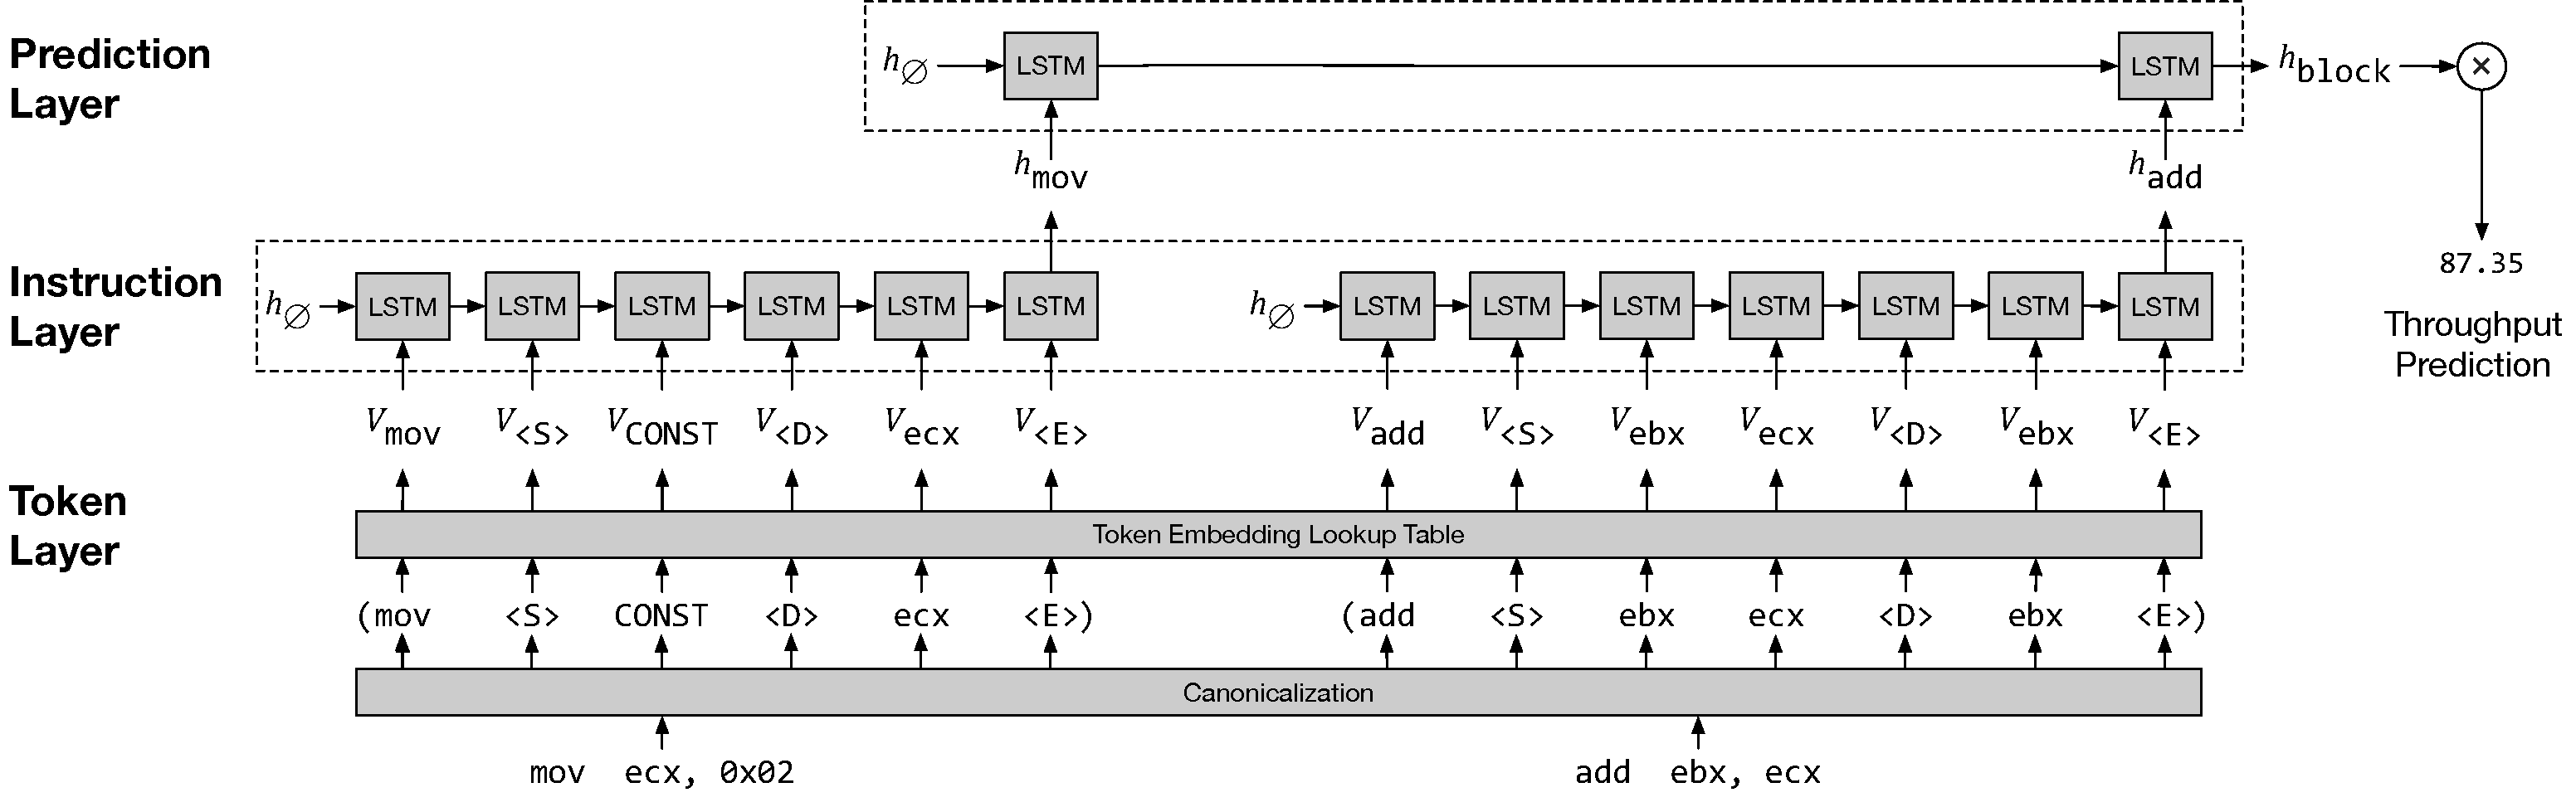
\includegraphics[width=\textwidth]{figures/diag_fullsystem.pdf}
  \vspace{-20pt}
  \caption{\tool{} System Architecture}
  \label{fig:overall}
\end{figure*}


\paragraph{Implementation Errors:}
Intel provides extensive documentation of its microarchitectural implementation that enables developers to build performance models for assembly code.
However, the sheer volume of implementation details makes it challenging to deliver a complete model.

Sequence (a) shows a single instruction sequence that zeros out the vector register \texttt{xmm0}.
Zeroing out registers is so common that Intel processors execute these instructions using a faster, optimized data path -- separate from the normal instruction execution path.
IACA closely predicts the measured value but llvm-mca's predictions are much farther off, because it does not model this optimization.

Sequence (b) shows a pair of \texttt{mov} instructions with a measured throughput of $103$.
IACA and LLVM both find an execution schedule which would predict a throughput of $100$ cycles; however, IACA also identifies a micro-op fusion opportunity, and therefore predicts $84$ cycles.
This optimization opportunity does not manifest in the observed timing numbers.

\tool{}, which is driven by actual performance data, learns to closely predict both of these values without any explicit error-prone encoding of Intel's optimizations.

\paragraph{Vendor Documentation Errors:}
The sheer volume of implementation details also means that Intel's documentation can be incorrect.
Tools that faithfully adhere to the documentation can therefore still be incorrect.
Sequence (c) is a short sequence with a data dependency that is bypassed within the processor pipeline: the \texttt{mov} instruction does not consume many additional clock cycles over that of \texttt{shl}.
The throughput of this basic block is therefore dominated by the throughput of \texttt{shl}.
However, the throughput value that Intel provides in its documentation (50 cycles) assumes that there are no dependencies.
Therefore, while IACA -- Intel's own tool -- closely predicts the value, llvm-mca is incorrect because it uses the dependency-free throughput value.
In comparison, \tool{} closely predicts the actual throughput because it works with actual performance data.
